\begin{figure}[h!]
	\centering
	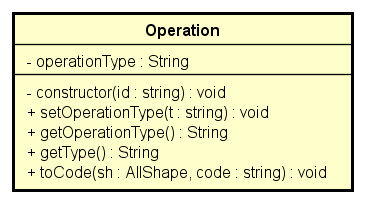
\includegraphics[scale=0.8]{res/sections/SpecificaFrontEnd/Services/Disegnetti/operation.png}
	\caption{Diagramma della classe Operation}
\end{figure}

\begin{itemize}
	\item \textbf{Descrizione:}\\
	
	\item \textbf{Utilizzo:}\\
	
	\item \textbf{Metodi:}
		\begin{itemize}
			\item \emph{-operationType : string}\\
    		Tipo di operazione
		\end{itemize}
	\item \textbf{Metodi:}
		\begin{itemize}
			\item \emph{-constructor(id: string)}\\
    		Costruttore della classe\\
    		\textbf{Parametri:}
    		\begin{itemize}
    			\item \emph{id: string}\\
    			Id dell'elemento
    		\end{itemize}
    		\item \emph{+setOperationType(t: string)}\\
    		Setta l'attributo operationType\\
    		\textbf{Parametri:}
    		\begin{itemize}
    			\item \emph{t: string}\\
    			Nuovo valore dell'attributo
    		\end{itemize}
    		\item \emph{+getOperationType()}\\
    		Ritorna il valore di operationType
    		\item \emph{+getType()}\\
    		Ritorna il tipo dell'operazione
    		\item \emph{+toCode(sh: AllShape, code: string)}\\
    		Converte la shape in codice\\
    		\textbf{Parametri:}
    		\begin{itemize}
    			\item \emph{sh: AllShape}\\
    			Shape da convertire
    			\item \emph{code: string}\\
    			Stringa di codice
    		\end{itemize}
    	\end{itemize}
\end{itemize}